\documentclass[aspectratio=169]{beamer}  
\usefonttheme{professionalfonts}
\usepackage{xeCJK}
\usepackage{fontspec}
\usepackage{graphicx}
\usepackage{listings}
\usepackage{xcolor}
\usepackage{indentfirst}
\usepackage{tikz}
\usepackage{amssymb}
\usepackage{amsthm}
\usepackage{amsmath}
\usepackage{tabularx}
\usepackage{hyperref}
\usepackage{comment}
\usepackage{ulem}
\usepackage{version}
\usepackage{thmtools}
\usepackage{qtree}
\usepackage{algpseudocode}
\usepackage{mathtools}
\usepackage{multicol}
\usepackage{xcolor}
\usepackage{diagbox}

\usefonttheme[onlymath]{serif}

\XeTeXlinebreaklocale "zh"
\XeTeXlinebreakskip = 0pt plus 1pt

\setsansfont{JetBrainsMono-Medium.ttf}
\setCJKmainfont[AutoFakeBold,AutoFakeSlant]{NotoSansTC-Regular.otf}
\usetikzlibrary{arrows,decorations.markings,decorations.pathreplacing}
\newenvironment{Hint}{\noindent\textbf{Hint.}}{}

\tikzstyle {graph node} = [circle, draw, minimum width=1cm]
\tikzset{edge/.style = {decoration={markings,mark=at position 1 with %
            {\arrow[scale=2,>=stealth]{>}}},postaction={decorate}}}

\lstset{
    language=C++,
    basicstyle=\ttfamily\tiny,
    commentstyle=\color{black!50},
    keywordstyle=\color{white!0!blue},
    stringstyle=\color{black!50!green},
    showspaces=false,
    showstringspaces=false,
    showtabs=false,
    tabsize=4,
    captionpos=b,
    breaklines=true,
    breakatwhitespace=false,
    escapeinside={\%*}{*)},
    morekeywords={*}
}

\AtBeginSection[]{
  \begin{frame}
  \vfill
  \centering
  \begin{beamercolorbox}[sep=8pt,center,shadow=true,rounded=true]{title}
    \usebeamerfont{title}\insertsectionhead\par%
  \end{beamercolorbox}
  \vfill
  \end{frame}
}

\title{數學 I}
\author{sam571128}
\date[附中延平競程讀書會]

\usetheme{Madrid}
\usecolortheme{default}
\setbeamertemplate{itemize items}[square]
\setbeamertemplate{enumerate items}[default]
\setbeamertemplate{blocks}[default]

\begin{document}

    %title
    \begin{frame}
        \titlepage
    \end{frame}
    
    %content
    \begin{frame}{目錄}
        \begin{itemize}
            \item 快速冪
            \item 質數篩
            \item 歐幾里得演算法
            \item 同餘、模運算
            \item 歐拉定理
            \item 中國剩餘定理
            \item 數論分塊
        \end{itemize}
    \end{frame}
    
    \section{快速冪 (Fast Exponentiation)}
    
    \begin{frame}{計算 $a^b$ 的答案?}
        \begin{itemize}
            \item 現在給你一個數字 $a$,如果想要找 $a^b$ 的話,你會怎麼做?
            \item<2-> 最直覺的作法,我們就直接一個數字一個數字往上乘就好了吧
            $$a^b = \underbrace{a \times a \times \cdots \times a}_{b \text{ times}}$$
            \item<3-> 不過這樣做,複雜度會是 $O(n)$ 的
            \item<3-> 有沒有更快的方式呢?
        \end{itemize}
    \end{frame}
    
    \begin{frame}{計算 $a^b$ 的答案?}
        \begin{itemize}
            \item 假設今天你要計算 $a^8$,你會怎麼算呢?
            \item<2-> 應該會很直覺的發現,雖然 $8$ 感覺起來要乘 $8$ 次
            \item<2-> 但你一定不會這樣做,而是
            $$a \rightarrow a^2 \rightarrow a^4 \rightarrow a^8$$
            \item<3-> 因為這樣子做,只需要乘 $3$ 次
        \end{itemize}
    \end{frame}
    
    \begin{frame}{計算 $a^b$ 的答案?}
        \begin{itemize}
            \item 那如果今天 $a$ 不是 $2$ 的次方呢?
            \item<2-> 仔細想一想,對於每個數字 $b$,其實我們都可以將其拆成二的次方的加總
            \item<3-> 例如:
            $$a^{15} = a^8 \times a^4 \times a^2 \times a^1$$
            \item<4-> 而你會發現,其實當我們將 $b$ 表示為二進位的形式後,做起來就一模一樣了!
        \end{itemize}
    \end{frame}
    
    \begin{frame}[fragile]{計算 $a^b$ 的答案?}
        \begin{itemize}
            \item 而用這樣的方式,我們可以在 $O(\log_2 n)$ 的時間完成計算
            \item 以下是參考程式碼
        \end{itemize}
        \begin{lstlisting}[language=C++,basicstyle=\ttfamily\small]
    int fastpow(int a, int b){
        int res = 0;
        while(b){
        if(b & 1) res = res * a % MOD;
            a = a * a % MOD;
            b >>= 1;
        }
        return res;
    }
        \end{lstlisting}
    \end{frame}
    
    \begin{frame}{計算 $a^b$ 的答案?}
        \begin{itemize}
            \item 也有另外一種方式
            \item<2-> 我們可以將次方拆成兩半,一路往下遞迴完成
            $$a^b = a^{\lfloor \frac{b}{2} \rfloor} \times  a^{\lfloor \frac{b}{2} \rfloor} \times a^{b \bmod 2}$$
            \item<3-> 以這樣的方式,我們可以寫出一個遞迴版本的快速冪
            \item<3-> 每次會將次方減半,因此時間複雜度也是 $O(\log_2 n)$
        \end{itemize}
    \end{frame}
    
    \begin{frame}[fragile]{計算 $a^b$ 的答案?}
        \begin{itemize}
            \item 以下是遞迴版本的參考程式碼
        \end{itemize}
        \begin{lstlisting}[language=C++,basicstyle=\ttfamily\small]
    int fastpow(int a, int b){
        if(b == 0)
            return 1;
        int x = fastpow(a,b/2);
        return x * x * fastpow(a,b%2);
    }
        \end{lstlisting}
    \end{frame}
    
    \begin{frame}[fragile]{計算 $a^b$ 的答案?}
        \begin{itemize}
            \item 在這個簡報裡,只要出現 $a^b$ 的話
            \item 我們將一律用 $O(\log n)$ 表示
        \end{itemize}
    \end{frame}
    
    \begin{frame}[fragile]{練習}
        \begin{block}{\href{https://cses.fi/problemset/task/1095}{CSES - Exponentiation}}
            請計算 $a^b \bmod 10^9+7$ 的答案。
        \end{block}
    \end{frame}
    
    \section{質數篩}
    
    \begin{frame}{找 $1 \sim n$ 的所有質數?}
        \begin{itemize}
            \item 現在,你想要知道 $1 \sim n$ 的範圍內有哪些數字是質數,你會怎麼做?
            \item<2-> 最直覺的想法,大概是直接跑過所有數字,並一一檢查每個數字是不是質數
            \item<3-> 一次檢查會需要花 $O(\sqrt{x})$ 的時間,因此檢查完所有數字就要 $O(n \sqrt{n})$!
            \item<4-> 效率實在是太低了
        \end{itemize}
    \end{frame}
    
    \begin{frame}[fragile]{找 $1 \sim n$ 的所有質數?}
        \begin{itemize}
            \item 發現到一個數字如果是質數,表示比他小的數字中,一定有他的因數
            \item<2-> 那我們換個方向思考,如果我們今天改成枚舉一個數字的倍數呢?
            \item<3-> 因此,我們得到了這樣的一個演算法
            \begin{lstlisting}[language=C++,basicstyle=\ttfamily\small]
bool isPrime[N];
void init(){
    fill(isPrime,isPrime+N,true);
    for(int i = 2; i < N; i++){
        if(isPrime[i]){
            for(int j = 2*i; j < N; j += i){
                prime[j] = false; 
            }
        }
    }
}
            \end{lstlisting}
        \end{itemize}
    \end{frame}
    
    \begin{frame}[fragile]{找 $1 \sim n$ 的所有質數?}
        \begin{itemize}
            \item 這個演算法的時間複雜度為 $O(\frac{n}{2}+\frac{n}{3} + \cdots)$
            \item 他的 bound 是 $O(n \log \log n)$ (有興趣的可以去看看維基百科)
            \item 而這個方法,名為「埃拉托斯特尼篩法 (Sieve of Erathosthenes)」
            \item 簡稱「埃氏篩」
        \end{itemize}
    \end{frame}
    
    \begin{frame}[fragile]{找 $1 \sim n$ 的所有質數?}
        \begin{itemize}
            \item 有沒有更快的做法呢?
            \item<2-> 有的!接下來要介紹的方法是可以在 $O(n)$ 的時間找到質數的方法
            \item<3-> 普遍被我們稱為「線性篩 (Linear Sieve)」的一種方法
            \item<4-> 我們會將每個數字的「最小質因數 (Least Prime Factor)」儲存下來
        \end{itemize}
    \end{frame}
    
    \begin{frame}[fragile]{找 $1 \sim n$ 的所有質數?}
        \begin{itemize}
            \item 概念是這樣,我們將所有質數存起來
            \item 接著依序去枚舉每個數字,並將數字與質數的乘積給刪除
            \item 這樣的做法,會發現每個數字最多只會被刪除一次!因此複雜度為 $O(n)$
        \end{itemize}
        \begin{lstlisting}[language=C++,basicstyle=\ttfamily\tiny]
    const int N = 1e5+5;
    int lpf[N];
     
    vector<int> primes;
    void init(){
        fill(lpf,lpf+N,1);
        for(int i = 2;i < N;i++){
            if(lpf[i]==1){
                lpf[i] = i;
                primes.push_back(i);
            }
            for(int x : primes){
                if(x*i > N) break;
                lpf[x*i]=x;
                if(x==lpf[i]) break;
            }
        }
    }
        \end{lstlisting}
    \end{frame}
    
    \begin{frame}{快速地質因數分解?}
        \begin{itemize}
            \item 在剛剛的線性篩的過程中,我們找出了每個數字的「最小質因數」
            \item 有了這個東西之後,其實可以利用他來做質因數分解
            \item 由於一個數字的相異質因數數量不會超過 $\lg n$ 個 
            \item 因此只要不停地把最小的質因數除掉,複雜度就會是 $O(\log n)$ 了!
        \end{itemize}
    \end{frame}
    
    \section{歐幾里得演算法 (輾轉相除法)}
    
    \begin{frame}[fragile]{找最大公因數?}
        \begin{itemize}
            \item 說到最大公因數這個東西,應該在國小或國中時都有學過各種不同的方法吧!
            \item 小時候會學到的方法可能會是短除法,不停地去尋找兩數共同的因數把他們除掉
            \item<2-> 這個方法找兩個數字 $a,b$ 的最大公因數的話,複雜度大概是 $O(\sqrt{max(a,b)})$
            \item<3-> 因此在長大後,你會學到另一種方法,也就是所謂的「輾轉相除法」
        \end{itemize}
    \end{frame}
    
    \begin{frame}{輾轉相除法}
        \begin{itemize}
            \item 大家應該以前也學過這個做法了吧,所以我們也來實際看一次吧!
        \end{itemize}
        \begin{center}
            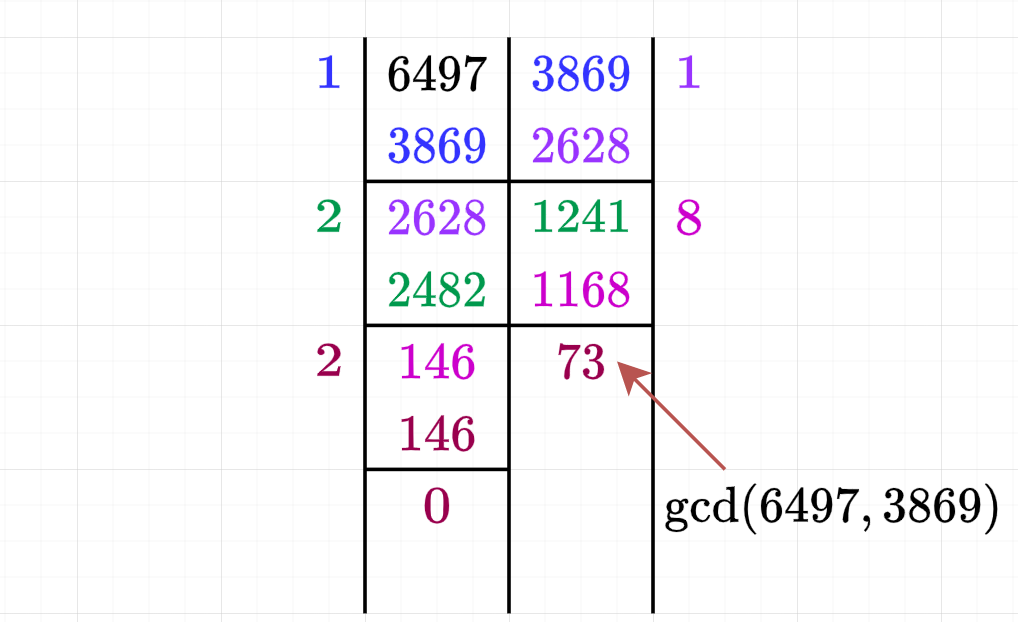
\includegraphics[scale=0.3]{images/euclidean_algorithm.png}
        \end{center}
    \end{frame}
    
    \begin{frame}{輾轉相除法}
        \begin{itemize}
            \item 這個方法做的事情是什麼呢?
            \item 實際上,這個方法利用到了一個性質
            $$\gcd(a,b) = \gcd(b, a \bmod b)$$
            \item 為什麼這會是對的呢,我們來簡單的證明一下
        \end{itemize}
    \end{frame}
    
    \begin{frame}{輾轉相除法}
        \begin{block}{輾轉相除法的證明}
            設 $m = \gcd(a,b)$,並將 $b$ 用除法原理寫成 $aq + (a\mod b)$,由於 $m \mid \gcd(a,b) \Rightarrow m \mid a, m \mid b$,因此,$m \mid (b-aq) \Rightarrow m \mid (a \bmod b)$。
        \end{block}
    \end{frame}
    
    \begin{frame}[fragile]{輾轉相除法}
        \begin{itemize}
            \item 有了這個性質之後,我們就可以很間單的寫出一個 $O(\log n)$ 的演算法!
            \begin{lstlisting}[language=C++,basicstyle=\ttfamily \small]
int gcd(int a, int b){
    if(b == 0) return 0;
    return gcd(b, a%b);
}
            \end{lstlisting}
        \end{itemize}
    \end{frame}
    
    \begin{frame}{貝祖定理}
        \begin{itemize}
            \item 既然講到最大公因數,我們也要來提一下一個小應用
            \item 檢查 $ax+by=c$ 是否有整數解!($a,b,c \in \mathbb{Z}$)
        \end{itemize}
        \begin{block}{貝祖定理}
            \begin{center}
                $ax+by=c$ 有整數解 $\iff$ $\gcd(a,b) | c$
            \end{center}
        \end{block}
    \end{frame}
    
    \begin{frame}{拓展歐幾里得演算法 (Extended GCD Algorithm)}
        \begin{alertblock}{拓展歐幾里得演算法 (Extended GCD Algorithm)}
            如果 $ax+by=c$ 有整數解,則 $bx'+(a \bmod b)y' = c$ 必有整數解 ($\gcd$ 不變)。 
            \vspace{2.5mm}
            原式可以轉換為 
            $$bx' + (a - b \Big \lfloor \dfrac{a}{b} \Big \rfloor)y' = c$$
            $$bx' + ay' - b \Big \lfloor \dfrac{a}{b} \Big \rfloor y' = c$$
            $$ay' + b (x' - \Big \lfloor \dfrac{a}{b} \Big \rfloor y') = c$$
            我們可以使用遞迴的方式找到一組 $(x,y)$ 的整數解
        \end{alertblock} 
    \end{frame}
    
    \begin{frame}[fragile]{拓展歐幾里得演算法 (Extended GCD Algorithm)}
        \begin{itemize}
            \item 實作方式如下
        \end{itemize}
        \begin{lstlisting}[language=C++,basicstyle=\ttfamily \small]
    pair<int,int> extgcd(int a, int b){
        if(b == 0) return {1,0};
        else if(a == 0) return {0,1};
        auto [x,y] = extgcd(b, a%b);
        return {y,x-a/b*y};
    }
        \end{lstlisting}
    \end{frame}
    
    \section{模運算、同餘}
    \begin{frame}{模運算}
        \setbeamercolor{block title}{use=structure,bg=green!50!black}
        \begin{block}{模運算 (Modulo Operation)}
            定義 $a \bmod b = r$,表示你可以找到一個 $q \in \mathbb{Z}$,使得 $a = bq+r$,而 $0 \le r < b$ 
            \begin{itemize}
                \item 等同於 C++ 當中的 \texttt{\%} 所做的事情
                \item 事實上,C++ 的 \texttt{\%} 做的事情就是這個,不同的點在於可能會有負數
                \item C++ 的 \texttt{\%} 定義為 $a \ \% \ b = a-b \times \Big \lfloor \frac{a}{b} \Big \rfloor$
                \item 由於 int 和 long long 都有固定的範圍,我們會利用 mod 來避免超出範圍
            \end{itemize}
        \end{block}
    \end{frame}
    
    \begin{frame}{模運算}
        \begin{alertblock}{模運算的性質}
            \begin{enumerate}
                \item $(a + b) \bmod n = ((a \bmod n) + (b \bmod n))\bmod n$
                \item $ab \bmod n = (a \bmod n) (b \bmod n) \bmod n$
                \item $\dfrac{a}{b} \bmod n \ne \dfrac{a \bmod n}{b \bmod n}$
            \end{enumerate}
        \end{alertblock}
        \begin{itemize}
            \item 這些性質可以簡單的用除法原理證明
            \item 這裡只放加法的證明,剩下的留給大家自己練習
        \end{itemize}
    \end{frame}
    
    \begin{frame}{模運算加法性質證明}
        令 $a = k_1n + r_1, \ b = k_2n + r_2$,而 $k_1,k_2 \in \mathbb{Z}$ and $0 \le r_1,r_2 < n$。根據 mod 的定義, $r_1 = a \bmod n, \ r_2 = b \mod n$.
        \begin{align*}
        (a+b) \bmod n &= (k_1n+r_1 + k_2n+r_2) \bmod n \\
                      &= (n(k_1+k_2) + r_1 + r_2) \bmod n \\
                      &= (r_1 + r_2) \bmod n \\
                      &= (a \bmod n) + (b \bmod n) \bmod n
        \end{align*}
        因此,我們證明了 $(a + b) \bmod n = ((a \bmod n) + (b \bmod n))\bmod n$.
    \end{frame}
    
    \begin{frame}{同餘}
        \setbeamercolor{block title}{use=structure,bg=green!50!black}
        \begin{block}{同餘 (Modular Congruence)}
            \begin{enumerate}
                \item $a \equiv b \pmod m$ 表示 $a \bmod m = b \bmod m$ 或 $(a-b) \bmod m = 0$
                \item 如果 $a \equiv b \pmod m$,則
                    \begin{itemize}
                        \item $a+c \equiv b+c \pmod m$
                        \item $a-c \equiv b-c \pmod m$
                        \item $ac \equiv bc \pmod m$
                        \item 不滿足 $a \div c \equiv b \div c \pmod m$
                    \end{itemize}
                \item 如果 $a \equiv b \pmod m, \ p \equiv q \pmod m$
                \begin{itemize}
                    \item $a+p \equiv b+q \pmod m$
                    \item $ap \equiv bq \pmod m$
                \end{itemize}
            \end{enumerate}
        \end{block}
    \end{frame}
    
    \begin{frame}{同餘}
        \begin{itemize}
            \item 這裡的證明與前面講過的十分相似,因此這裡也不多作證明
            \item 不過你一定會想,既然在有模運算的系統下,不能直接做除法
            \item 那我們有沒有什麼方法可以幫助我們達到這一點呢?
            \item 答案是有的!也就是接下來要介紹的「模反元素」
        \end{itemize}
    \end{frame}
    
    \begin{frame}{同餘 (Modular Congruence)}
        \setbeamercolor{block title}{use=structure,bg=green!50!black}
        \begin{block}{模反元素 (Modular Inverse)}
            對於一個元素 $x$,在 $\bmod \ m$ 的系統下,$x^{-1}$ 為滿足 $xx^{-1}\equiv 1 \pmod m$ 的數字,我們稱 $x^{-1}$ 為 $x$ 的「模反元素」或「模逆元」。而並不是對於所有 $x$ 皆存在一個模反元素。模反元素存在 $\iff$ $x$ 與 $m$ 互質。
        \end{block}
    \end{frame}
    
    \begin{frame}{同餘 (Modular Congruence)}
        \begin{itemize}
            \item 有了模逆元之後,模運算下的除法會寫成 $ab^{-1}$ 來表示 $a$ 除以 $b$ 後的答案
            \item 因此,我們會需要找出一個數字的模逆元
            \item 以下我們提供三種可以找模逆元的方法
        \end{itemize}
    \end{frame}
    
    \begin{frame}{模反元素找法}
        \begin{itemize}
            \item 費馬小定理 (只有在 $m$ 是質數時可以使用)
            \item 建表法 (只有在 $m$ 是質數時可以使用)
            \item 拓展歐幾里得定理 (又稱 extgcd,當 $gcd(a,m) = 1$ 時可以使用)
        \end{itemize}
    \end{frame}
    
    \begin{frame}{模反元素找法一 - 費馬小定理 (Fermat's Little Theorem)}
        \begin{alertblock}{費馬小定理 (Fermat's Little Theorem)}
            當 $p$ 是質數時,對於任一個整數 $a$,滿足 $a^{p-1} \equiv 1 \pmod p$
        \end{alertblock}
    \end{frame}
    
    \begin{frame}{模反元素找法一 - 費馬小定理 (Fermat's Little Theorem)}
        \begin{block}{證明}
            \begin{enumerate}
                \item 當 $p \mid a$ 時,必滿足 $a^p \equiv a \pmod p$。
                \item 對於 $a,2a,\ldots,(p-1)a$,這些數字除以 $p$ 的餘數必一一對應到 $1,2,\ldots,p-1$,可以用反證法證明。因此 $(p-1)!a^{p-1} \equiv a \times 2a \times \cdots \times (p-1)a \equiv (p-1)! \pmod p$。得 $a^{p-1}\equiv 1 \pmod p$
            \end{enumerate}
        \end{block}
    \end{frame}
    
    \begin{frame}{模反元素找法二 - 建表法}
        假設我們想要計算 $i$ 在 $\mod \ p$ ($p$ 必須是質數) 下的模反元素,推導過程如下
        \begin{align*}
            p - i \times \Big \lfloor \dfrac{p}{i} \Big \rfloor&= p \bmod i \\
            p - i \times \Big \lfloor \dfrac{p}{i} \Big \rfloor &\equiv p \bmod i \pmod p \\
            p \times i - i \times \Big \lfloor \dfrac{p}{i} \Big \rfloor &\equiv p \bmod i \pmod p \\
            i(p - \Big \lfloor \dfrac{p}{i} \Big \rfloor)(p \bmod i)^{-1} &\equiv 1 \pmod p \\
            (p - \Big \lfloor \dfrac{p}{i} \Big \rfloor)(p \bmod i)^{-1} &\equiv i^{-1} \pmod p 
        \end{align*}
    \end{frame}
    
    \begin{frame}{模反元素找法二 - 建表法}
        \begin{itemize}
            \item 因此我們得到了這個公式
            $$i^{-1} \pmod p \equiv (p - \Big \lfloor \dfrac{p}{i} \Big \rfloor)(p \bmod i)^{-1}$$
            \item<2-> 可以使用遞迴的方式直接往下找答案,
            \item<2-> 經過實測,在 $\mod$ 是 $10^9+7$ 或 $998244353$ 的情況下,複雜度幾乎是 $O(\log n)$
            \item<3-> 這個方法還可以在 $O(n)$ 的時間建出 $1 \sim n$ 的模逆元! 
        \end{itemize}
    \end{frame}
    
    \begin{frame}{模反元素找法三 - 拓展歐幾里得定理 (Extended GCD)}
        當我們要找 $a$ 在 $\bmod \ m$ 下的模反元素,若滿足 $gcd(a,m)=1$,則我們可以列出
        $$aa^{-1} + bm = 1$$
        使用拓展歐幾里得找 $a^{-1}$ 即可
    \end{frame}
    
    \begin{frame}{歐拉函數 (Euler Phi Function)}
        \begin{block}{歐拉函數 (Euler Phi Function)}
            對於正整數 $n$,定義 $\phi(n)$ 為小於等於 $n$ 且與 $n$ 互質的正整數數量。
            \begin{enumerate}
                \item 對於一個質數 $p$,$\phi(p) = p-1$
                \item 若 $a,b$ 互質,則 $\phi(ab) = \phi(a) \phi(b)$ (積性函數)
                \item $a^{\phi(m)} \equiv 1 \pmod m$ (歐拉定理)
                \item 假設 $n=p_1^{\alpha_1}p_2^{\alpha_2}\dots p_k^{\alpha_k}$,則 $\phi(n) = n \prod_{i=1}^k (1-\frac{1}{p_i})$
            \end{enumerate}
        \end{block}
    \end{frame}
    
    \begin{frame}{中國剩餘定理 (Chinese Remainder Theorem)}
        \begin{itemize}
            \item 當你遇到了以下這樣的問題
            \item 中國剩餘定理可以幫助我們找到所有滿足以下式子的解
        \end{itemize}
        \begin{equation*}
            \quad \left\{ \begin{matrix} x \equiv a_1 \pmod {m_1} \\ x \equiv a_2 \pmod {m_2} \\ x \equiv a_3 \pmod {m_3} \\ \vdots \\ x \equiv a_n \pmod {m_n} \end{matrix} \right.
        \end{equation*}
    \end{frame}
    
    \begin{frame}{中國剩餘定理 (Chinese Remainder Theorem)}
        這個問題有兩種解法:
        \begin{enumerate}
            \item 使用通解的形式找到答案
            \item 使用拓展歐幾里得算法計算答案 (比賽中常用的方式)
        \end{enumerate}
        第一種作法的話,我們會快速帶過,在競程上比較常使用第二種方式
    \end{frame}
    
    \begin{frame}{中國剩餘定理 (Chinese Remainder Theorem)}
        \begin{alertblock}{構造通解的方式}
            假設 $m_1, m_2, \dots, m_n$ 互質
            \begin{enumerate}
                \item 設 $M = m_1 m_2 \dots m_n = \prod_{i=1}^n m_i$,而 $M_i = M/m_i$
                \item 設 $t_i \equiv M_i^{-1} \pmod{m_i}$,意即 $t_i$ 是 $M_i$ 的模反元素  
                \item 則通解會是 $x \equiv a_1t_1M_1 + a_2t_2M_2 + \dots + a_n t_n M_n \equiv \sum_{i=1}^n a_i t_i M_i \pmod M$
            \end{enumerate}
        \end{alertblock}
    \end{frame}
    
    \begin{frame}{中國剩餘定理 (Chinese Remainder Theorem)}
        我們依序合併每個式子,先從最前面的兩個開始
        $$\quad \left\{ \begin{matrix} x \equiv a_1 \pmod {m_1} \\ x \equiv a_2 \pmod {m_2} \end{matrix} \right.$$
        則我們可以知道對於兩個整數 $k_1, k_2$
        $$\quad \left\{ \begin{matrix} x = k_1m_1 + a_1 \\ x = k_2m_2 + a_2 \end{matrix} \right.$$
        合併兩個式子,我們會得到
        $$k_1m_1 + a_1 = k_2m_2 + a_2$$
        移項一下會得到
        $$m_1k_1 - m_2k_2 = a_2-a_1$$
    \end{frame}
    
    \begin{frame}{中國剩餘定理 (Chinese Remainder Theorem)}
        接著我們可以使用 extgcd,找到一組 $k_1, k_2$ 的解 $(k_1', k_2')$ \\
        \vspace{5mm}
        再將 $k_1$ 代入 $x = a_1 + m_1k_1$ 的式子當中,兩式就合併成 
        $$x \equiv a_1 + m_1 k_1 \pmod {\text{lcm}(m_1,m_2)}$$
        利用這個方法將 $n$ 個式子合併即可得到答案
    \end{frame}
    
    \section{數論分塊}
    
    \begin{frame}{數論分塊}
        \begin{block}{經典題}
            給你一個數字 $n$,請找到以下算式的答案:
            $$\sum_{i=1}^n \lfloor \frac{n}{i} \rfloor$$ 
            \begin{itemize}
                \item $1 \le n \le 10^{12}$
            \end{itemize}
        \end{block}
        \begin{itemize}
            \item<2-> 範圍好大喔,要怎麼處理阿
        \end{itemize}
    \end{frame}
    
    \begin{frame}[fragile]{數論分塊}
        \begin{itemize}
            \item 遇到這種問題時,其實我們可以嘗試看看暴力
        \end{itemize}
        \begin{lstlisting}[language=C++,basicstyle=\ttfamily\small]
    int n;
    cin >> n;
    for(int i = 1; i <= n; i++){
        cout << n/i << "\n";
    }
        \end{lstlisting}
    \end{frame}
    
    \begin{frame}[fragile]{數論分塊}
        \begin{center}
            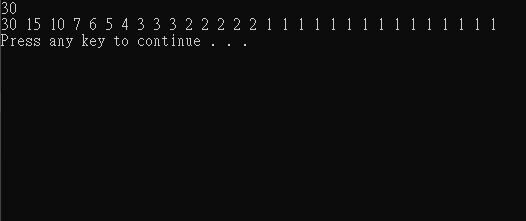
\includegraphics[scale=0.7]{images/number_theory_block.png}
        \end{center}
    \end{frame}
    
    \begin{frame}[fragile]{數論分塊}
        \begin{itemize}
            \item 欸? 數字好像會連在一起出現欸
            \item 那如果我們有了 $\lfloor \frac{n}{i} \rfloor$ 的值
            \item 如果我們可以知道最大的 $j$ 除起來也會是這個值
            \item 那我們是不是可以優化這樣的做法呢?
        \end{itemize}
    \end{frame}
    
    \begin{frame}[fragile]{數論分塊}
        \begin{itemize}
            \item 可以證明,對於一個數字 $k = \lfloor \frac{n}{i} \rfloor$
            \item 最大能夠使得 $k = \lfloor \frac{n}{j} \rfloor$ 的 $j$
            \item 可以經由以下算式計算出來
            $$\Big \lfloor \frac{n}{k} \Big \rfloor$$
        \end{itemize}
    \end{frame}
    
    \begin{frame}[fragile]{數論分塊}
        \begin{itemize}
            \item 而我們也可以發現,$\lfloor \frac{n}{i} \rfloor$ 其實最多只有 $2 \sqrt{n}$ 種不同的值
            \item 證明:
            \begin{enumerate}
                \item 對於 $i \le \sqrt{n}$,$\lfloor \frac{n}{i} \rfloor$ 最多只有 $\sqrt{n}$ 種不同的數字
                \item 對於 $i > \sqrt{n}$, $\lfloor \frac{n}{i} \rfloor \le \sqrt{n}$ 最多也只有 $\sqrt{n}$ 種不同的數字
            \end{enumerate}
            \item 因此這個做法的複雜度為 $O(\sqrt{n})$
        \end{itemize}
    \end{frame}
    
\end{document}